\section{Training a Judge for Selection}
\label{sec:training}

Outcome-labelled verdict training rewards a judge for predicting whether an attempt's answer is right.

On our pools, $56\%$ of the label entropy is question difficulty:
\[
H(Z)=0.91 \text{ bits} = \underbrace{I(Z;X)}_{0.51} + \underbrace{\mathbb E[H(p_x)]}_{0.40}.
\]
With 4 attempts per question, $53\%$ of wrong attempts come from questions with no right attempt. These carry no
within-question contrast. On a globally balanced set like Phase~2's, a judge that knows only $p_x$ earns $86\%$ verdict
reward.

\paragraph{Proposition 3 (pointwise--selection misalignment).}
Suppose the judge sees one attempt with a difficulty-like cue $x_b=s_b z_x+e_b$ that varies between attempts of the
same question (length, for example), and a within cue $x_w=dZ+e_w$. For a score $\theta_b x_b+\theta_w x_w$,
\begin{equation}
d'_{\text{within}}=d\,\theta_w/\sqrt{\theta_b^2+\theta_w^2}.
\end{equation}
\begin{itemize}
\item When $P(Z\mid x)$ varies with $x$, the pointwise-optimal $\theta_b$ is positive and strictly lowers
  within-question discrimination.
\item Class rebalancing changes only the intercept.
\item Under \emph{per-question balance} ($P(Z{=}1\mid x)=\frac12$ for every $x$), $x_b$ carries no information and
  $\theta_b=0$. The initial gradient on any question-only feature is then $\mathbb E[(\frac12-Z)\varphi(x)]=0$.
\end{itemize}

In a finite-sample learning model with 64-dimensional features, 900 questions and 1,024 training examples, per-question
balanced or pairwise data raise within-question AUROC from $0.67$ to $0.74$ while \emph{lowering} pooled AUROC from
$0.86$ to $0.74$ (Figure~\ref{fig:training}). Judge checkpoints must therefore be compared on within-question AUROC,
not pooled AUROC.

Per-question pairs scale as $N(N-1)\,\mathbb E[p(1-p)]$ per question: $1.07$ at $N=4$ and $21.4$ at $N=16$.

\begin{figure}[t]
\centering
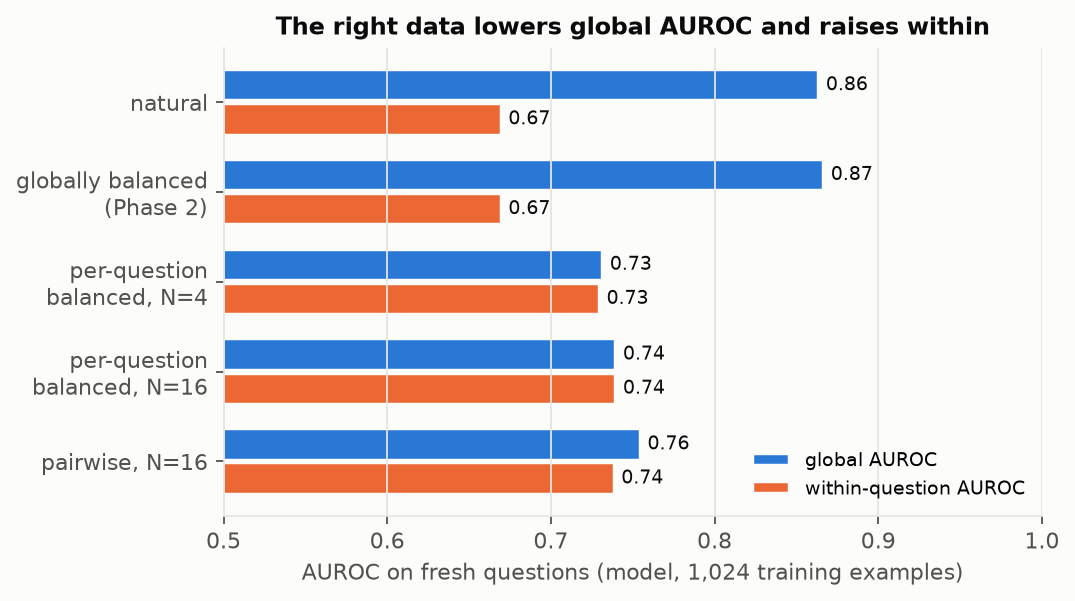
\includegraphics[width=\columnwidth]{figures/fig4_training_regimes.png}
\caption{Learning model (1,024 examples from 900 questions). Per-question balanced and pairwise data trade pooled
AUROC for within-question AUROC.}
\label{fig:training}
\end{figure}
